\documentclass{article}
\usepackage{graphicx,url}
\usepackage[brazil]{babel}
\usepackage[utf8]{inputenc}
\usepackage{enumerate}
\usepackage{tabularx}
\usepackage{multirow}
\usepackage{amsmath}
\usepackage[table,xcdraw]{xcolor}

\title{Proposta de Pesquisa: \\
Ferramentas para Business Report com Suporte à XBRL
}
\author{Vagner Clementino \\ 
       \url{vagnercs@dcc.ufmg.br}}
\date{Setembro de  2015}


\begin{document}

\maketitle

\section{Introdução}
\label{sec:intro}

To do.

\section{Justificativa}
\label{sec:contexto}

Tendo em vista determinação da Secretaria do Tesouro Nacional, órgão
vinculado ao  Ministério da Fazenda do Brasil, que definiu o XBRL como
padrão para o envio de relatórios de prestação de contas pelos entes
federativos (estados e municípios), surge a necessidade por parte
destes últimos do \textit{desenvolvimento ou aquisição} de sistemas de
informação capazes de criar, processar e enviar informações no formato
XBRL. Como o objetivo de deixar mais claro o contexto no qual esta
necessidade se apresenta analisemos a seguir um cenário em que o
problema se apresenta descrito como \textit{storytelling}:
\\
\\
\begin{center}
\fbox{
\begin{minipage}{28em}
%\textit{
Arnaldo é gerente de projeto em uma empresa responsável pelo
desenvolvimento de sistemas para uma prefeitura de médio porte no
estado de Minas Gerais. Ele foi informado pela diretoria da empresa
que devido à mudanças legais, definidas Secretaria do Tesouro
Nacional, as prestações de contas da prefeitura para o governo federal
deverá ser realizada em um novo formato denominado XBRL, acrônimo de
eXtensible Business Reporting Language. Arnaldo sabe que os sistemas
de informações à serviço da prefeitura já são capazes de enviar
relatório aos órgãos fiscalizadores nos formatos CSV (Comma-separated
values) e xls (Microsoft Excel Binary File Format). Após uma análise
profunda do problema, o gerente entende que há dois caminhos possíveis para atender a demanda da prefeitura:

\begin{enumerate}[(i)]
\item Adquirir uma ferramenta de terceiros que suporte à prestação de contas no formato XBRL;
\item Desenvolver na própria empresa um  sistema de informação de informação que possibilite a prestação de conta no formato requirido mas que também possibilite a geração nos formatos já utilizados;
\end{enumerate}

Naturalmente ambas as soluções possuem \textit{prós e contras}. Caso a
organização opte por \textit{adquirir} (caminho (i)) ela não precisará
enfrentar o risco do baixo conhecimento que existe atualmente na
equipe com relação ao assunto \textit{XBRL}. Todavia, o sistema
comprado por terceiros poderá não atender todos aos requisitos
necessários sendo necessário uma customização posterior, algo cuja
experiência anteriores demonstraram que implicam em um maior custo
para a organização. De outra forma, a criação de um projeto (solução
ii) possui uma maior probabilidade de aderência aos requisitos, em
contrapartida possui os desafios naturais da construção de um sistema
do zero.

A fim de subsidiar a decisão de qual caminho seguir, Arnaldo realiza
uma busca na Internet de comparativo entre ferramentas para Business
Report com suporte à XBRL, contudo, os resultados se mostram
incipientes. Ele novamente utiliza uma ferramenta de busca com
objetivo de pesquisar sobre boas práticas e lições apreendidas que
possa ajudar na construção de ferramentas para Business Report e novamente fica decepcionado com os dados retornado. Arnaldo sente-se frustrado por não conseguir referências que o ajude em definir entre a solução (i) e (ii).
%}
\end{minipage}
}
\end{center}

Ao analisarmos o problema descrito no estudo de caso do gerente
Arnaldo, verifica-se que existe a necessidade por parte das
organizações, especialmente as entidades públicas, de referências de
qualidade sobre o assunto de \textit{XBRL}. Trabalhos com este enfoque
poderiam \textit{subsidiar a tomada de decisão} por parte dos gestores
públicos. Por exemplo, para aqueles inclinados pela \textit{solução
  (i)} poderiam utilizar uma  \textit{Revisão Sistemática da
  Literatura} - SLR (do inglês Systematic Literature Review) que
avaliasse as ferramentas para Business Report que dão suporte ao
XBRL. No caso daqueles que optarem pela  \textit{solução (ii)} a
estratégia empírica que melhor lhe daria suporte seria um
\textit{Survey} que poderia coletar dados de diferentes partes
interessadas (stakeholders) sobre o processo de prestação de contas
das diversas prefeituras do país afim de avaliar as melhores práticas
e lições aprendidas no desenvolvimento e utilização de sistema de
informação para aquela finalidade.

Cabe ressaltar neste ponto que existe na literatura, especialmente da
Engenharia de Software, a utilização de Revisão Sistemática da
Literatura (SLR) e Survey como sinônimos. Na realidade a SLR pode se
considerado um subtipo de Survey. Todavia, com o objetivo de enviar
qualquer tipo de mal entendido consideramos SLR e Survey como duas
estratégias empíricas \cite{wohlin2012experimentation} distintas, as
quais serão formalmente definidas a seguir.

Um \textbf{Survey} é um sistema para coletar informações de ou sobre
\textit{pessoas} para descrever, comparar ou explicar seus
conhecimentos, atitudes e comportamento \cite{fink2003survey}. Um
Survey geralmente é conduzido em retrospectiva, ou seja, tem como
objetivo avaliar a utilização por um determinado período de uma
ferramenta ou técnica \cite{kitchenham2009systematic}. Outra
característica marcante dos Survey é que estes são aplicados em uma
amostra de uma população visando derivar conclusões sobre a mesma\cite{robson2002real}.

\section{Objetivos do Trabalho}
\label{sec:objetivos}

O trabalho ora proposto tem como objetivo desenvolver dois trabalhos
empíricos sobre o assunto \textit{XBRL}. A primeira parte consiste no
desenvolvimento de uma \textit{Revisão Sistemática da Literatura -
  SLR} sobre ferramentas de \textit{Business Report} com suporte ao
padrão XBRL. O público alvo do referido trabalho serão pesquisadores,
programadores, gestores que precisam de uma fonte de informação
independente que avaliasse as soluções existentes no mercado. A partir
dos dados obtidos da \textit{SLR} seria possível, por exemplo, propor
novas Ferramentas ou mesmo melhorias nas existentes.

A segunda parte do trabalho seria a realização de \textit{Survey} com
pessoas que participam diretamente do processo de prestação de contas
entre entes federativos. Dentre estas pessoas podemos citar
contadores, desenvolvedores, gestores e etc que poderiam fornecer
detalhes sobre o atual contexto daquele processo. Os dados fornecidos
por aqueles profissionais pode ajudar no desenvolvimento de
ferramentas que efetivamente atendam as necessidades de seus usuários.

\section{Revisão Sistemática da Literatura}
\label{sec:rsl}

Uma Revisão Sistemática da literatura (SLR), por se tratar de método
científico, deve seguir uma sequência rigorosa de passos a fim de
alcançar os seus objetivos. Alguns diretrizes orientam como sequências
fundamentais no processo de desenvolvimento de uma
SLR\cite{keele2007guidelines}, dentre outras: 
\begin{itemize}
  \item especificar uma ou mais sentenças de buscas que serão
    inseridas nas ferramentas de busca com o objetivo de recuperar os
    estudo preliminares que serão utilizados na revisão;
  \item definir um conjunto de \textit{questões de pesquisa} que
    servirão de norte na condução do trabalho;
 \item  desenvolver um protocolo que definirá os procedimentos a serem adotados durante a revisão, ele servirá como um guia para a condução da revisão. 
\end{itemize}

Nas próximas subseções iremos detalhar cada um dos passos descrito anteriormente.
\subsection{Sentenças de Busca}
\label{subsec:setences}

Como a revisão proposta tem como principal objetivo ser uma referência para aqueles interessados em avaliar ferramentas de Business Report com suporte à XBRL, naturalmente sentenças como ``XBRL", ``tools", ``Business Report"\footnote{Inicialmente será utilizado apenas as sentenças na língua inglesa} se mostram como boas candidatas. 

A fim de avaliar qual sentença de busca possibilitaria um conjunto de
estudos preliminares com maior relevância para o trabalho, foi
realizada um estudo prévio utilizando a ferramenta de pesquisa Google
Schoolar\footnote{\url{https://scholar.google.com.br/}}. O estudo é
bastante simples, consistindo apenas em registrar o total de artigos
recuperados quando realizado uma pesquisa com uma sentença $S_n$
qualquer. Não foi utilizado qualquer tipo de filtro na busca (como por
exemplo "por data") e os resultados foram classificados por
relevância. Apesar do simplicidade deste estudo ele se mostra como um
bom ponto de partida para definirmos a sentenças de buscam que
futuramente irão possibilitar a recuperação dos estudos preliminares. A tabela \ref{tab:sentencas} exibe as sentenças utilizadas bem como o total de artigos recuperados.


\begin{table}[]
\centering
\resizebox{\textwidth}{!}{%
\begin{tabular}{clc}
\rowcolor[HTML]{EFEFEF} 
{\bf Código da Sentença} & \multicolumn{1}{c}{\cellcolor[HTML]{EFEFEF}{\bf Sentença}} & {\bf Total de Artigos}     \\ \hline
\multicolumn{1}{|c|}{$S_1$} & \multicolumn{1}{l|}{“XBRL”}                                & \multicolumn{1}{c|}{15000} \\ \hline
\multicolumn{1}{|c|}{$S_2$} & \multicolumn{1}{l|}{“XBRL tools”}                          & \multicolumn{1}{c|}{3710}  \\ \hline
\multicolumn{1}{|c|}{$S_3$} & \multicolumn{1}{l|}{“XBRL Business Report tools”}          & \multicolumn{1}{c|}{4110}  \\ \hline
\multicolumn{1}{|c|}{$S_4$} & \multicolumn{1}{l|}{“XBRL tools marketing”}                & \multicolumn{1}{c|}{1290}  \\ \hline
\multicolumn{1}{|c|}{$S_5$} & \multicolumn{1}{l|}{“XBRL Business Report software tools”} & \multicolumn{1}{c|}{2970}  \\ \hline
\end{tabular}
}
\caption{Total de artigos por sentença}
\label{tab:sentencas}
\end{table}

Como pode ser observado a sentença $S_1$ é a consulta mais genérica que poderia ser feita sobre no contexto da XBRL, contudo, é retornado um total de $15000$ um valor relativamente pequeno comparado ao total de artigos retornados ao realizar consultas com o termo ``XML' por exemplo\footnote{A consulta por XML retorna aproximadamente $3 \times 10^{6}$ artigos}.

Não obstante a sentença $S_6$ se mostrou satisfatória tanto pelo total
de artigos recuperados bem como pela relevância dos mesmo, auferida
pela inspeção manual de alguns resultados. Visando avaliar o impacto
de restringir o ano de publicação na sentença $S_6$ foi realizada um
novo conjunto de buscas no qual foi utilizado o critério de seleção
``artigos a parte do ano''.  Os resultados são exibidos na Figura \ref{fig:graph_artigos_ano}{}.

\begin{figure}[h] 
\label{fig:graph_artigos_ano}
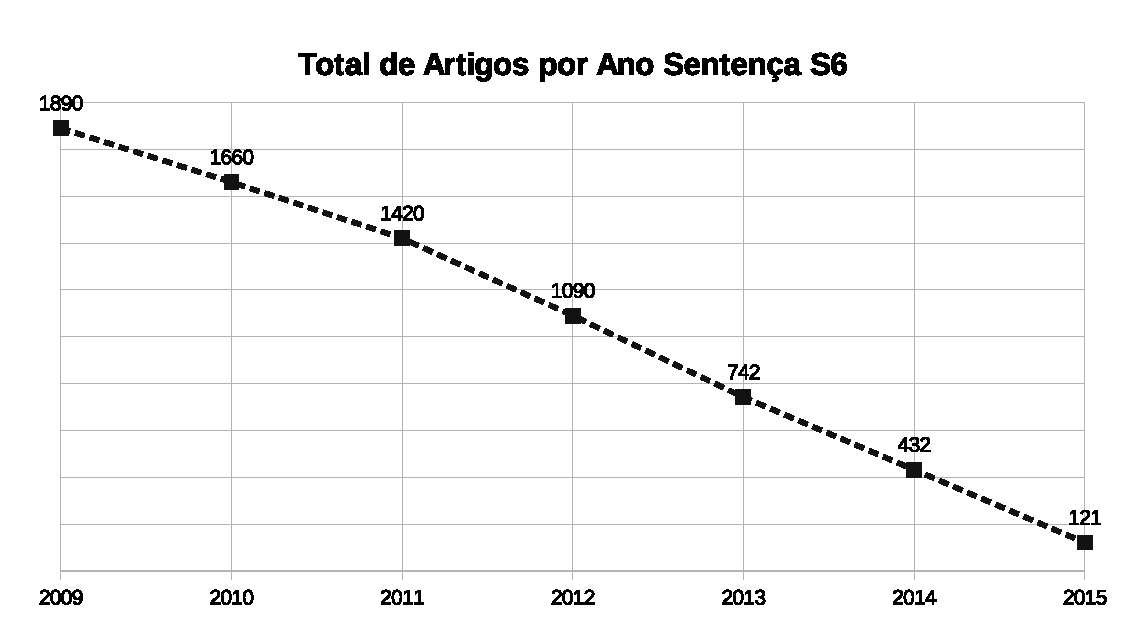
\includegraphics[width=8cm]{../img/graph_01.eps}
\caption{Total de artigo a partir de determinado ano para a sentença $S_6$}
\centering
\end{figure}

A Figura \ref{fig:graph_artigos_ano} mostra conforme esperado a
redução do número de artigos quanto se limita o período de
pesquisa. Em uma análise preliminar pode-se afirmar que a utilização
de artigos publicados a partir de 2012 consegue englobar uma massa de
artigos suficiente para um estudo ponto de partida. Posteriormente,
mediante o Protocolo da Revisão serão definidos critérios para
inclusão e exclusão de ababalho na revisão. Os detalhes destas
diretrizes estão detalhadas na Subseção \ref{subsec:protocol}.

\subsection{Questões de Pesquisa}
\label{subsec:research_question}

In work.

\subsection{Protocolo de Desenvolvimento da Revisão}
\label{subsec:protocol}

Aguardando definições.

\section{Survey com Stakeholders}
\label{sec:survey}

Avaliando viabilidade.

\section{Cronograma}
\label{sec:cronograma}


\section{Próximas Etapas}
\label{sec:proximas_etapas}

Aguardando definições.

\medskip

\bibliographystyle{unsrt}%Used BibTeX style is unsrt
\bibliography{../bib/propostaref}

\end{document}
